\documentclass[12pt]{article}
\usepackage{geometry}
\geometry{a4paper}


\usepackage{color}
\usepackage{hyperref}
\usepackage{amsmath}
\usepackage{amsfonts}
\usepackage{amssymb}
\usepackage{graphicx}
\usepackage{tcolorbox}
\usepackage{listings}
\usepackage{here}
\usepackage{txfonts}
\usepackage{algorithm}
\usepackage{algorithmic}
\usepackage{siunitx}
\usepackage{xcolor}
\usepackage{ascmac}
%\usepackage{fancybx}

\lstset {language = c++,
  basicstyle = \ttfamily \scriptsize,
  commentstyle = \textit,
  frame = tRBl,
  framesep = 5pt,
  showstringspaces = false,
  numbers = left,
  stepnumber = 1,
  numberstyle = \tiny,
  tabsize = 2,
  keywordstyle = \bfseries \color{blue},
  stringstyle=\color{magenta},
  commentstyle=\color{red},
  morecomment=[l][\color{red}]{\#}
  showstringspaces=false, % don't mark spaces in strings
}
\newcommand{\bi}[1]{\mathbf{#1}}
\newcommand{\bs}[1]{\boldsymbol{#1}}  % bold for greek characters
\newcommand{\bbR}{\mathbb{R}}

\author{Nobuyuki Umetani}

\title{Rigid Body Dynamics \footnote{This is just a note to keep in mind what I learned when I was MSc student.}}



\begin{document}
\maketitle
\tableofcontents


%%%%%%%%%%%%%%%%%%%%%%%%%%%%%%%%%%%%%%%%%%%%%%%%%%%%%%%%%%%%%%%%%%%%%%%%%%%%%%%%
\section{Angular velocity and parametrization of 3D rotation}

In this section, we discuss about variation and time derivative of a rotation matrix.

\subsection{Variation of a rotation matrix}

Let's investigate the variation of the rotation matrix. Rotation matrix $\bi{R}$ satisfies $\bi{R}^T \bi{R} = \bi{I}$. By computing the derivative as follows:
%
\begin{eqnarray}
&&  \bi{R}^T \bi{R} = \bi{I}\\
&\Leftrightarrow& \delta(\bi{R}^T\bi{R}) = \delta\bi{I} = 0\\
&\Leftrightarrow& \delta\bi{R}^T\bi{R} + \bi{R}^T\delta\bi{R} = 0\\
&\Leftrightarrow& \delta\bi{R}^T\bi{R} + (\delta\bi{R}^T\bi{R})^T = 0\\
&\Leftrightarrow& sym(\delta\bi{R}^T\bi{R}) = 0
\end{eqnarray}

Therefore $\delta\bi{R}^T\bi{R}$ can be seen to be an antisymmetric matrix because its symmetric component is 0. Since it is an antisymmetric matrix, it can be expressed as follows using the appropriate vector $\delta\bi{\Theta}$ and tilde symbol.


\begin{equation}
\delta\Theta = vect(\delta\bi{R}^T\bi{R}) \;\Leftrightarrow\; \delta\tilde{{\Theta}} = \bi{R}^T\delta\bi{R} \;\Leftrightarrow\; \delta\bi{R} = \bi{R}\delta\tilde{{\Theta}}
\end{equation}

Although the rotation matrix has various parameterization methods and it was very complicated, it can be seen that the variation itself can be expressed simply as a vector. Actually, there is another kind of display of the variation vector of the rotation matrix. Start from the variations of the identity matrix as before.

\begin{eqnarray}
&&  \bi{R} \bi{R}^T = \bi{I}\\
&\Leftrightarrow& \delta(\bi{R}\bi{R}^T) = \delta\bi{I} = 0\\
&\Leftrightarrow& \delta\bi{R}\bi{R}^T + \bi{R}\delta\bi{R}^T = 0\\
&\Leftrightarrow& \delta\bi{R}\bi{R}^T + (\delta\bi{R}\bi{R}^T)^T = 0\\
&\Leftrightarrow& sym(\delta\bi{R}\bi{R}^T) = 0
\end{eqnarray}


Therefore, $\delta\bi{R}\bi{R}^T$ has symmetric component of 0, which shows that it is an antisymmetric matrix. Since it is an antisymmetric matrix, it can be expressed as follows using the appropriate vector $\delta\bi{\theta}$ and tilde symbol.

\begin{equation}
\delta\theta = vect(\delta\bi{R}\bi{R}^T) \;\Leftrightarrow\; \delta\tilde{\theta} = \delta\bi{R}\bi{R}^T \;\Leftrightarrow\; \delta\bi{R} = \delta\tilde{\theta}\bi{R}
\end{equation}
\ \ \ \

It was found that the variance of the rotation matrix is ​​vectorized by the two vectors $\delta\theta,\delta\Theta$ as follows.

\begin{tcolorbox}[title=two vector notations for variational rotation]
\begin{eqnarray}
\delta\bi{R} &=& \bi{R}\delta\tilde{\Theta}\\
\delta\bi{R} &=& \delta\tilde{\theta}\bi{R}
\end{eqnarray}
\end{tcolorbox}

The meaning of $\bi{\Theta}$ and $\bi{\theta}$ means that each change in rotation is expressed as being rotated by $\bi{R}$ after slight rotation by $\bi{\Theta}$ in the initial placement or it is expressed by saying that $\bi{\theta}$ was slightly rotated in the current arrangement rotated by $\bi{R}$ It corresponds to that. It is customary to display vectors in initial placement in capital letters and vectors in current placement in lower case letters.

\begin{eqnarray}
\delta\tilde{\Theta} = \bi{R}^T\delta\tilde{\theta}\bi{R}\\
\delta\tilde{\theta} = \bi{R}\delta\tilde{\Theta}\bi{R}^T
\end{eqnarray}




\subsection{Angular Velocity Vector}

Let's examine the differential $\dot{\bi{R}}$ of the rotation matrix. Suppose that a certain vector $\bi{X}$ in the initial arrangement moves like $\bi{x}=\bi{R}\bi{x}$ by the rotation matrix $\bi{R}$. Taking time differentiation of both sides yields $\dot{\bi{x}}=\dot{\bi{R}}\bi{x}$, it can be seen that the differential $\dot{\bi{R}}$ of the rotation matrix expresses the relationship between the vector at the initial arrangement and the speed at the current arrangement. \\

By the way, it is a differentiation $\dot{\bi{R}}$ of this rotation matrix, but it can be vectorized by exactly the same argument as the differential $\delta\bi{R}$ of the rotation matrix of the former subchapter (it can be considered that $\delta$ is a time differential operator). The time derivative of the rotation matrix is ​​displayed by a certain vector $\Omega,\omega$ as follows.

\begin{tcolorbox}[title=two vector notation of rate of rotation change]
\begin{eqnarray}
\dot{\bi{R}} &=& \bi{R}\tilde{\Omega}\\
\dot{\bi{R}} &=& \tilde{\omega}\bi{R}
\end{eqnarray}
\end{tcolorbox}


In this document, we will call $\Omega$ the angular velocity vector in the initial arrangement and $\omega$ the angular velocity vector in the current arrangement.


\section{Equation of Motion for Rigid Bodies Derived using the Hamilton Principle}

\subsection{mass and the center of gravity}

The total mass $m$ of the rigid body is as follows.

\begin{equation}
m = \int_v \rho dv
\end{equation}

Also, the center of gravity $\bi{x}_g$ is expressed as follows using this

\begin{equation}
\bi{x}_g = \frac{1}{m}\int_v\rho \bi{x} dv
\end{equation}

Here, in a rigid body, the following expression holds.

\begin{tcolorbox}[title=material point positioin on a rigid body]
\begin{equation}
\bi{x}(t) = \bi{x}_g(t) + \bi{R}(t)\{\bi{x}(0) - \bi{x}_g(0)\}
\end{equation}
\end{tcolorbox}

\begin{figure}
\begin{center}
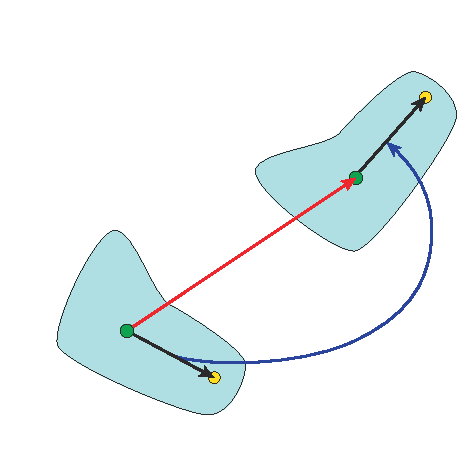
\includegraphics[width=80mm]{images/RigidTransRot.pdf}
\caption{rigid body translation and rotation}
\end{center}
\end{figure}



Here, there is no volume change in the minute volume as follows.

\begin{equation}
dv = \left(\det\bi{R}\right)dV = dV
\end{equation}

Therefore, from the mass conservation law at the mass point,

\begin{equation}
\rho(\bi{x}(t)) = \rho(\bi{x}(0))
\end{equation}

Is satisfied. That is, there is no change in density at a certain material point. Of course, the mass of the rigid body also does not change over time as follows.

\begin{equation}
m = \int_v \rho(\bi{x}(t)) dv = \int_V \rho(\bi{x}(0))dV
\end{equation}


\subsection{Mechanical energy}

The mechanical energy of the rigid body is as follows.

\begin{equation}
{\cal K} = \frac{1}{2}\int_v \rho \dot{\bi{x}}^T \dot{\bi{x}}dv
\end{equation}

For simplicity, let $\bi{X}$ be the position with the center of gravity in the initial placement as follows.

\begin{equation}
\bi{X} = \bi{x}(0) - \bi{x}_g(0)
\end{equation}

Then the position of the mass point of the rigid body can be written as follows.

\begin{equation}
x(t) = x_g(t) + \bi{R}(t)\bi{X}
\end{equation}

The time differentiation of both sides is as follows.

\begin{equation}
\bi{\dot{x}} = \dot{\bi{x}}_g + \dot{\bi{R}}\bi{X}
\end{equation}

When this is substituted into the above equation, it becomes as follows.

\begin{eqnarray}
\dot{\bi{x}}^T \dot{\bi{x}}
&=& (\dot{\bi{x}}_g + \dot{\bi{R}}\bi{X})^T(\dot{\bi{x}}_g + \dot{\bi{R}}\bi{X}) \\
&=& \dot{\bi{x}}^T_g \dot{\bi{x}}_g + \bi{X}^T\dot{\bi{R}}^T\dot{\bi{x}}_g + \dot{\bi{x}}_g\bi{\dot{R}}\bi{X} + (\dot{\bi{R}}\bi{X})^T(\dot{\bi{R}}\bi{X})\\
&=& \dot{\bi{x}}^T_g \dot{\bi{x}}_g + 2\dot{\bi{x}}_g\bi{\dot{R}}\bi{X} + (\dot{\bi{R}}\bi{X})^T(\dot{\bi{R}}\bi{X})
\end{eqnarray}

Using this,

\begin{eqnarray}
{\cal K}
&=&
\left(\frac{1}{2}\int_v \dot{\bi{x}}^T_g \dot{\bi{x}}_g dv\right)   +  \left(\frac{1}{2}\int_v 2\dot{\bi{x}}_g\bi{\dot{R}}\bi{X}dv\right)   +   \left(\frac{1}{2}\int_v(\dot{\bi{R}}\bi{X})^T(\dot{\bi{R}}\bi{X})dv\right)\\
&=& {\cal K}_1 + {\cal K}_2 + {\cal K}_3
\end{eqnarray}

You can write like this. We will proceed with calculations in order for each item below \ \

\textbf{ Calculation in first term} 
%
Calculate for the first term. This term represents the dynamical energy in the movement of the center of gravity.

\begin{equation}
{\cal K}_1 = \frac{1}{2}\int_v\rho \dot{\bi{x}}_g^T\bi{\dot{x}}_g dv = \left(\frac{1}{2}\int_v\rho dv\right)\dot{\bi{x}}_g^T\bi{\dot{x}}_g  = \frac{1}{2}m \dot{\bi{x}}_g^T\bi{\dot{x}}_g
\end{equation}

\textbf{Calculation of second term} 
%
The second term of the dynamic energy is as follows.

\begin{eqnarray}
{\cal K}_2
&=& \frac{1}{2}\int_v\rho 2\dot{\bi{x}}_g\bi{\dot{R}}\bi{X} dv = \dot{\bi{x}}_g\bi{\dot{R}}\int_V\rho \bi{X} dV\\
&=& \dot{\bi{x}}_g\bi{\dot{R}}\int_V\rho\left(\bi{x}(0)-\bi{x}_g(0)\right)dV\\
&=& \dot{\bi{x}}_g\bi{\dot{R}}\int_V\rho\{m\left(\frac{1}{m}\int_V\rho\bi{x}(0)dV\right)-\bi{x}_g(0)\int_V\rho dV\} \\
&=& \dot{\bi{x}}_g\bi{\dot{R}}\{m\bi{x}_g(0)-m\bi{x}_g(0)\}\\\;\;\;\; = 0
\end{eqnarray}

It can be seen that this term can be ignored. The reason that the second term disappears is that it shows the transformation and rotation with the center of gravity as the base point to express the deformation of the rigid body. \\

\textbf{Calculation in the third term} 
The third term of mechanical energy was as follows.

\begin{equation}
{\cal K}_3 = \frac{1}{2}\int_V\rho(\dot{\bi{R}}\bi{X})^T(\dot{\bi{R}}\bi{X})dV
\end{equation}

Here, the differentiation of the rotation matrix can be transformed as follows.

\begin{equation}
\dot{\bi{R}}\bi{X} = \bi{R}\tilde{\bi{\Omega}}\bi{X} = -\bi{R}\tilde{\bi{X}}\bi{\Omega}
\end{equation}

When this is substituted into the above equation,

\begin{eqnarray}
(\dot{\bi{R}}\bi{X})^T(\dot{\bi{R}}\bi{X})
&=& (-\Omega^T\tilde{\bi{X}}^T\bi{R}^T)(-\bi{R}\tilde{\bi{X}}\bi{\Omega})\\
&=& \Omega^T\tilde{\bi{X}}^T\tilde{\bi{X}}\bi{\Omega}
\end{eqnarray}

Here, the moment of inertia $\bi{J}$

\begin{tcolorbox}[title=moment of inertia]
\begin{equation}
\bi{J} = \int_V \rho\tilde{\bi{X}}^T \tilde{\bi{X}}dV = \int_V \rho(||\bi{X}||^2\bi{I} - \bi{X}\bi{X}^T )dV
\end{equation}
\end{tcolorbox}

Substituting into the above equation,

\begin{equation}
{\cal K}_3 = \frac{1}{2}\int_V\rho \Omega^T\tilde{\bi{X}}^T\tilde{\bi{X}}\bi{\Omega}dV  = \frac{1}{2}\Omega^T\{\int_V\rho \tilde{\bi{X}}^T\tilde{\bi{X}}dV\}\bi{\Omega}  = \frac{1}{2}\Omega^T \bi{J} \bi{\Omega}
\end{equation}


Together, the mechanical energy ${\cal K}$ of the rigid body is as follows,

\begin{tcolorbox}[title=kinetic energy]
\begin{equation}
{\cal K} = \frac{1}{2}(m\dot{\bi{x}}_g^T \bi{\dot{x}}_g + \Omega^T \bi{J} \bi{\Omega})
\end{equation}
\end{tcolorbox}

\subsection{Potential Energy}

Energy due to volume force and energy due to surface force can be considered as potential energy. 
%
Examples of the volume force include gravity, electromagnetic force, pressure as an example of surface force. 
%
Here, consider the volume force, especially the potential energy due to a constant gravity force $\bi{g}$.

\begin{eqnarray}
{\cal V}
&=& -\int_v \rho\left(\bi{x}(t)-\bi{x}(0)\right)^T \bi{g} dv\\
&=& -(\bi{x}_g(t)-\bi{x}_g(0))^Tm\bi{g}
\end{eqnarray}

Therefore, the potential energy is represented by the displacement of the center of gravity.
%
The variations are as follows.
%
\begin{equation}
\delta{\cal V} = -\delta\bi{x}_g^T(t)m\bi{g}
\end{equation}


\subsection{Equation of motion}
Derive the equation of motion using the Hamiltonian principle. Using the Hamiltonian principle, you can choose arbitrary variables for the equation, so you can easily describe the motion including the rotation like a rigid body.
%
Let's assume that restraint condition $\Phi=0$ is imposed on exercise. $\Phi$ is assumed to be differentiable once for the degree of freedom of translation and rotation of a rigid body.
%
Lagrangian ${\cal L}$ is defined as follows. Where $\lambda$ is the Lagrangian multiplier multiplier.

\begin{equation}
{\cal L} = {\cal K} - {\cal V} -\lambda^T \Phi
\end{equation}

We define the quantity ${\cal I}$ called the action as follows.

\begin{equation}
{\cal I} = \int_{t_1}^{t_2} {\cal L} dt
\end{equation}

The Lagrangian principle is that the motion from time $t_1$ to $t_2$ has an extreme value when the variation in $t_1,t_2$ is 0. In other words,

\begin{equation}
\delta{\cal I}= 0
\end{equation}

Is satisfied. Let us derive the equation of motion of the rigid body by actually calculating this action for the rigid body.


\subsubsection{Variation of kinetic energy}

The variation of the dynamic energy is as follows

\begin{eqnarray}
\delta {\cal K}
&=& \delta\dot{\bi{x}}_g^T m \dot{\bi{x}}_g + \delta \Omega^T \bi{J} \Omega\\
&=& \delta\dot{\bi{x}}_g^T m \dot{\bi{x}}_g + (\delta \dot{\Theta} + \tilde{\Omega}\delta\Theta)^T \bi{J} \Omega\\
&=& \frac{d}{dt}\{\delta \bi{x}_g^T m \bi{x}_g\} - \delta\bi{x}_g^T m\ddot{\bi{x}}_g   + \frac{d}{dt}\{\delta\Theta^T \bi{J}\Omega\} - \delta\Theta^T\bi{J}\dot{\Omega} + \delta\Theta^T\tilde{\Omega}^T\bi{J}\bi{\Omega}\\
&=& \frac{d}{dt}\{\delta \bi{x}_g^T m \bi{x}_g + \delta\Theta^T \bi{J}\Omega\} - \delta\bi{x}_g^T m\ddot{\bi{x}}_g  - \delta\Theta^T(\bi{J}\dot{\Omega}+\tilde{\Omega}\bi{J}\Omega)
\end{eqnarray}

Now, the variations are as follows.

\begin{eqnarray}
\int_{t_1}^{t_2}\delta{\cal K}dt
&=& \left[\delta \bi{x}_g^T m \bi{x}_g + \delta\Theta^T \bi{J}\Omega\right]_{t_1}^{t_2}\;\; - \int_{t_1}^{t_2}\left[\delta\bi{x}_g^T m\ddot{\bi{x}}_g  + \delta\Theta^T(\bi{J}\dot{\Omega}+\tilde{\Omega}\bi{J}\Omega)\right]dt\\
&=& - \int_{t_1}^{t_2}\delta\bi{x}_g^T m\ddot{\bi{x}}_g  + \delta\Theta^T(\bi{J}\dot{\Omega}+\tilde{\Omega}\bi{J}\Omega)dt
\end{eqnarray}
%
Here, we used $\delta\bi{x}_g = 0$ and $\delta\bi{\Theta} = 0$ at time $t_1,t_2$.

\subsubsection{Variation of constraint}

The motion of the rigid body is represented by the position $\bi{x}_g$ and the rotation $\bi{R}$ of the center of gravity. Let's calculate this variance assuming that constraints are imposed on this.

\begin{equation}
\lambda^T \Phi = \delta\lambda^T\Phi +\lambda^T\delta\Phi
\end{equation}

Now looking closely at $\delta\Phi$ in the second term on the right side of the above equation,

\begin{eqnarray}
\delta\Phi
&=&  \Phi(\delta\bi{x}_g,\bi{R}) + \Phi(\bi{x}_g,\delta{\bi{R}})\\
&=& \Phi(\delta\bi{x}_g,\bi{R}) + \Phi(\bi{x}_g,\bi{R}\delta\tilde{\Theta})\\
&=& \frac{\partial \Phi}{\partial \bi{x}_g}\delta\bi{x}_g + \frac{\partial\Phi}{\partial\Theta}\delta\Theta
\end{eqnarray}


\subsection{Derivation of equations of motion by variation of action}

\begin{eqnarray}
\delta{\cal I}
&=& \delta\int_{t_1}^{t_2} {\cal L} dt\\
&=& \delta\int_{t_1}^{t_2} {\cal K} - {\cal P} - \lambda^T\Phi dt\\
&=& - \int_{t_1}^{t_2}\delta\bi{x}_g^T m\ddot{\bi{x}}_g  + \delta\Theta^T(\bi{J}\dot{\Omega}+\tilde{\Omega}\bi{J}\Omega)dt + \int_{t_1}^{t_2}\delta\bi{x}_g^Tm\bi{g}dt  \\
&& - \int_{t_1}^{t_2}\delta\lambda^T\Phi  + \lambda^T\left\{\frac{\partial \Phi}{\partial \bi{x}_g}\delta\bi{x}_g + \frac{\partial\Phi}{\partial\Theta}\delta\Theta\right\}dt\\
&=& \int_{t_1}^{t_2}\delta\bi{x}_g^T\left\{-m\ddot{\bi{x}}_g+m\bi{g}-\left(\frac{\partial \Phi}{\partial \bi{x}_g}\right)^T\lambda\right\}dt\\
&&   - \int_{t_1}^{t_2}\delta\Theta_g^T\left\{\bi{J}\dot{\Omega}+\tilde{\Omega}\bi{J}\Omega+\left(\frac{\partial\Phi}{\partial\Theta}\right)^T\lambda\right\}dt   -   \int_{t_1}^{t_2}\delta\lambda^T\Phi dt
\end{eqnarray}

Since this is true for all $\delta\bi{x}_g$, $\delta\bi{\Theta}$, $\delta\lambda$,

\begin{eqnarray}
\left\{\begin{array}{rrl}
m\ddot{\bi{x}}_g + \left(\frac{\partial \Phi}{\partial \bi{x}_g}\right)^T\lambda &=& m\bi{g}\\
\bi{J}\dot{\Omega}+\tilde{\Omega}\bi{J}\Omega+\left(\frac{\partial\Phi}{\partial\Theta}\right)^T\lambda &=& 0\\
\Phi &=& 0\end{array}\right.
\end{eqnarray}

Is satisfied.

\if0 
\section{What I referred to}

\ cite {Crisfield 199705}, \ cite {Japan Society of Mechanical Engineers 200708}, \ cite {Japan Society of Mechanical Engineers 200603}, \ cite {Tajima 200611}, \ cite {McCauley 199705}

\ cite {EmanPhysicsAnalytical}, \ cite {PhysicsKeyTailAnalytic}

\ bibliographystyle {tipsj}
\ bibliography {.. / main}
\fi

\end{document}
